

\section{Model klasyczny - podejście matematyczne}
Model neuronu \cite{Korbicz1994},  można rozpatrywać jako przetwornik sygnałów ciągłych, bardziej zbliżonych do logiki rozmytej (fuzzy logic) niż boolowskiej. Sygnały wejściowe i wyjściowe  przyjmują wartości z określonych zakresów, co implikuje działania na  wartościach zmiennoprzecinkowych kodowanych najczęściej w standardzie IEEE 754 i odpowiadających im typom \textit{float} lub \textit{double}. Na wejście neuronu podawana jest pewna liczba \(m\) sygnałów wejściowych \(x_1\) ... \(x_m\), natomiast na wyjściu pojawia się tylko jeden sygnał wyjściowy \(z\). Odpowiedź neuronu to jedna wartość, a odpowiedź warstwy to zbiór wartości (wektor). Odpowiedź warstwy typu „softmax” jest wprost wektorem rozkładów prawdopodobieństwa przynależności do klas.

\begin{figure}[ht]
	\centering 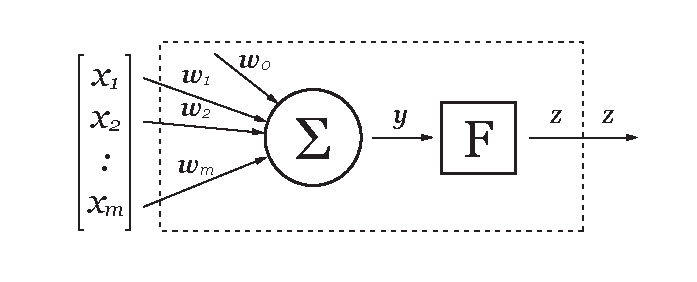
\includegraphics{rysunki/rys1_1.jpg} 
	\caption{Model sztucznego neuronu~\cite{Korbicz1994} }
	\label{rys:modelsztucznegoneuronu2a}
\end{figure}

Samo przetwarzanie polega na wyznaczeniu sumy ważonej sygnałów wejściowych, a następnie na wyliczeniu wartości funkcji aktywacji:

\begin{equation}
       y = \sum^{m}_{i=1} x_i*w_i - \theta,
       z = F(y)
\end{equation}
gdzie: \(x_i\) - i-ty sygnał wejściowy,
       \(w_i\) - i-ta waga w neuronie,
       \(\theta\) - energia aktywacji,
       F - funkcja aktywacji,
       z - wielkość sygnały wyjściowego neuronu.

Przy podstawieniu: \(z_0=1\) oraz \(w_0=-\theta\) wzór przyjmuje wygodniejszą postać:
\begin{equation}
       y = \sum^{m}_{i=0} x_i*w_i
\end{equation}


Neurony zorganizowane są w warstwy w taki sposób, by te należące do jednej warstwy miały dostęp do tego samego wektora wejściowego X. Sygnał wyjściowy każdego neuronu to pojedyncza wartość \(z_j\), zaś na sygnał wyjściowy warstwy składają się sygnały wszystkich neuronów należących do tej warstwy i tworzą wektor Z. Liczbę neuronów w warstwie oznaczamy \(n\), zatem liczba wymiarów wektora Z to także \(n\).

\begin{equation*}
       Z = \left[
       \begin{matrix}
                    z_1,\\
                    z_2,\\
                    :\\
                    z_n\\
                \end{matrix}
       \right]
\end{equation*}


W najprostszych układach neurony z jednej warstwy nie komunikują się między sobą.

W zapisie wektorowym mamy:
\begin{equation*}
       X = \left[
       \begin{matrix}
                    x_0 = 1,\\
                    x_1 ...\\
                    :\\
                    x_m ...\\
       \end{matrix}
       \right] 
\end{equation*}
\begin{equation*}
       W = \left[
            \begin{matrix}

            W_1 & W_2 & W_3 \\
            \left[
                        \begin{matrix}
                             w_{0}\\
                             w_{1}\\
                             w_{m}\\
                        \end{matrix}
            \right] 
            &
                        \left[
                        \begin{matrix}
                             w_{0}\\
                             w_{1}\\
                             w_{m}\\
                        \end{matrix}
            \right] 
            &
                        \left[
                        \begin{matrix}
                             w_{0}\\
                             w_{1}\\
                             w_{m}\\
                        \end{matrix}
            \right] 
            
 
            \end{matrix}
       \right]\\
\end{equation*}

\begin{equation*}
       z_1=F(W_1.*X)
\end{equation*}
\begin{equation*}
       Z=F(W^T*X)
\end{equation*}

Rozpisujemy mnożenie macierzy przez macierz \(W^T*X\) jak poniżej:
\begin{equation*}
       \begin{matrix}
                     & 
                     \left[
                        \begin{matrix}
                             x_{0}\\
                             x_{1}\\
                             x_{m}\\
                        \end{matrix}
                    \right]
                    &
                    \\
                     
                     
                     
                     \left[
                        \begin{matrix}
 \text{   } w_{10} \text{  }, \text{   } w_{11} \text{   } , \text{   } w_{1m} \text{   }\\
 \text{   } w_{20} \text{  }, \text{   } w_{21} \text{   } , \text{   } w_{2m} \text{   }\\
 \text{   } w_{n0} \text{  }, \text{   } w_{n1} \text{   } , \text{   } w_{nm} \text{   }\\ 
                        \end{matrix}
                        \right]
                        
                   & 
                   \left[
                        \begin{matrix}
     x_{0}*w_{10} + x_{1}*w_{11} + x_{m}*w_{1m} \\
     x_{0}*w_{20} + x_{1}*w_{21} + x_{m}*w_{2m} \\
     x_{0}*w_{n0} + x_{1}*w_{n1} + x_{m}*w_{nm} \\
                        \end{matrix}
                    \right] 
                    &=\left[
                        \begin{matrix}
     y_{0} \\
     y_{1} \\
     y_{m} \\
                        \end{matrix}
                    \right]
                    \\
       \end{matrix}
\end{equation*}
 w którym \(X\) jest wektorem wejściowym, x\(_i\) jest i-tym sygnałem wejściowym, w\(_i\) jest i-tą wagą, w\(_{ji}\) jest i-tą wagą j-tego neuronu,  W\(_j\) oznacza zapis wag jako wektor, zaś  W oznacza macierz wag. 
 \newline Symbol .* oznacza mnożenie Hadamarda czyli mnożenie pierwszego elementu z~pierwszym, drugiego z drugim itd. Zapis \(X^T\) oznacza  transpozycję macierzy lub wektora. Zapis \(W^T*X\) oznacza mnożenie macierzowe \(X^T\) przez W. \textbf{Aby wyliczyć odpowiedz jednej warstwy musimy wykonać \(m*n\) mnożeń i \((m-1)*n\) dodawań oraz musimy wyliczyć \(n\) razy wartości funkcji \(F(y_j)\).}


\subsection{Funkcje aktywacji}

\begin{figure}[ht]
	\centering 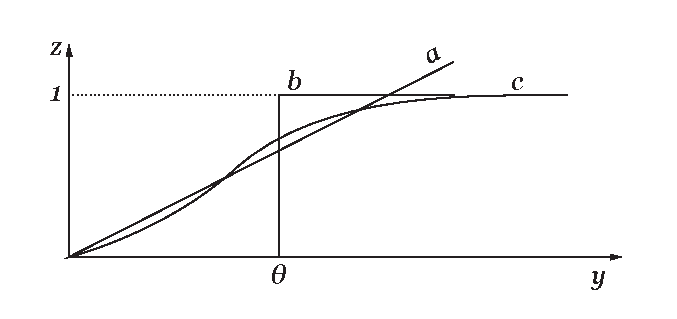
\includegraphics{rysunki/rys1_2.jpg} 
	\caption{Funkcje aktywacji}
	\label{rys:funkcje aktywacji}
\end{figure}

Sygnał \(y\) przetwarzany przez blok aktywacji F może być opisany różnymi funkcjami.

\begin{itemize}
    \item Może być to np. prosta funkcja liniowa (a):
    \begin{equation}
       z = ky , \text{gdzie \(k\) jest zadanym stałym współczynnikiem.}
    \end{equation}
    

\item ReLU - funkcja liniowa, która w części dodatniej ma współczynnik k=1, oraz współczynnik k=0 w części ujemnej: 
    \begin{equation}
       z = F(y) = y^+ = max(0,y) = z \Biggl\{
                \begin{matrix}
                    x \text{ jeśli } y>0,\\
                    0 \text{ jeśli } y\leq 0,
                \end{matrix} 
    \end{equation} 

    \item Funkcja skokowa Heaviside’a, skok jednostkowy (b):
        \begin{equation}
            y = H(z) = \Biggl\{
                \begin{matrix}
                    1 \text{ jeśli } y>\theta,\\
                    0 \text{ jeśli } y\leq\theta,
                \end{matrix}
        \end{equation}

            \item Funkcja bipolarna:
        \begin{equation}
            y = sgn(z) = \Biggl\{
                \begin{matrix}
                    1 \text{ jeśli } y>\theta,\\
                    -1 \text{ jeśli } y\leq\theta,
                \end{matrix}
        \end{equation}
       
\item Funkcja logistyczna (sigmodalna) (c):
        \begin{equation}
            z = \frac {1} { 1 + exp (- \beta y) }, \text{ 
  dla \(\beta\)=1 pochodna: } \frac {\partial z}{\partial y}= z(1-z)
        \end{equation}
\end{itemize} 


\newpage
\subsection{Proces uczenia}

\begin{figure}[h]
	\centering 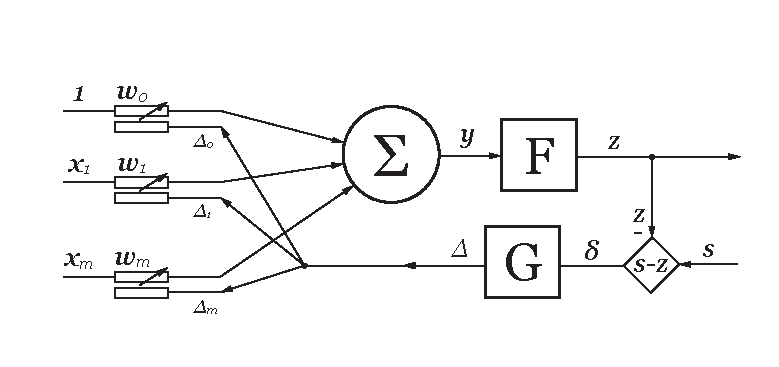
\includegraphics{rysunki/rys1_3.jpg} 
	\caption{Proces uczenia elementu perceptronowego}
	\label{rys:procesuczeniaelementu}
\end{figure}

Proces uczenia pojedynczego neuronu polega na:
\begin{itemize}
\item obliczeniu wartości sygnału wyjściowego \(y\);
\item obliczeniu wartości sygnału wyjściowego \(z=F(y)\);

\item porównaniu wektora wyjściowego \(z\) z wartością oczekiwaną \(s\) oraz obliczenie różnicy \(\delta=s-z\);

\item zależnie od metody uczenia wyznaczenia wartości \(\Delta = G(\delta)\);
\item wyznaczenie wielkości poprawek dla poszczególnych wag \(\Delta_i\);
\item aktualizacja wagi: \(w(k+1)=w(k)+\Delta w(k)\).
\end{itemize}

Możemy to  opisać wzorem:
\begin{equation}
       w(k+1) = w(k) + G(s-z) 
\end{equation}
gdzie: \(w(k+1)\) jest wartością uaktualnioną, \(w(k)\) wartością przed aktualizacją. Funkcja \(G(\delta)\) jest funkcją, na podstawie której obliczamy wielkości poprawek.

\subsection{Algorytm propagacji wstecznej}
W algorytmie propagacji wstecznej \cite{Korbicz1994}, \cite{russell2023}, wysyłamy do warstwy wejściowej próbkę danych X, wyjście  warstwy łączy się z wejściem następnej, a~wynik przetwarzania warstwy poprzedniej jest wysyłany do~warstwy następnej i tak aż do wyjścia. Wynik odczytany z~warstwy wyjściowej porównujemy z oczekiwaną wartością wyjściową. 
Różnica tych wartości stanowi błąd \( \delta \). Wartość błędu jest przesyłana w kierunku odwrotnym, czyli od warstwy wyjściowej aż do wejściowej i na podstawie wielkości błędu korygowane są wielkości wag neuronów w kolejnych warstwach. 
\newline
Aby proces był optymalny, zakładamy pewną funkcję straty „Loss” „\({L}\)” której parametrami są wagi warstw, wektory wejściowe i powiązane z nimi oczekiwane wartości wyjściowe. Wartość tej funkcji określa wielkość błędu odpowiedzi sieci dla pojedynczego sygnału wejściowego X. Chcemy znaleźć takie wagi warstw, dla których suma błędów dla wszystkich próbek w serii (zwanej epoką) będzie jak najmniejsza. Zapiszemy 

\begin{equation*}
      Loss(S,Z)=Loss(S,F(Y))=Loss(S,F(x_1*w_1,x_2*w_2...x_m*w_m)) 
\end{equation*} 

\begin{equation}
      \sum _{n=1} ^N {\mathbbm{L}(S, F(y))}= \sum _{n=1} ^N {\mathbbm{L}(s1_1, ... ,s_m, F(x_1*w_1, ... , x_m*w_m ))} 
\end{equation} 
gdzie \(\mathbbm{L}\) jest funkcją straty, \(F\) jest funkcją aktywacji, a X jest wektorem wejściowym, S oczekiwaną odpowiedzią, zaś n liczbą próbek X.

Z analizy matematycznej wiemy, że w miejscach, w których występuje extremum funkcji, jej pierwsze pochodne się zerują. Dla funkcji wielu zmiennych metoda obliczania punktów zerowania pochodnych jest niepraktyczna, wygodniejsza jest iteracyjna metoda  \textit{spadku gradientowego}, w której korygujemy wagi o pewien krok w kierunku największego spadku funkcji \(\mathbbm{L}\). W tym przypadku korekty wyniosą:
\begin{equation}
w_{ji} = w_{ji} + \eta * \frac{\partial}{\partial w_j}\mathbbm{L}       
\end{equation}
\newline
Jeśli przyjmiemy miarę \(\mathbbm{L}\) jako miarę błędu kwadratowego \(\mathbbm{L} = (s-z)^2 = (s-F(y))^2 \)  
\newline
wówczas:
\begin{equation*}
\frac{\partial}{\partial w_j}\mathbbm{L}  = 
        \frac{\partial}{\partial F}\mathbbm{L} 
        * \frac{\partial}{\partial y_i}F 
        * \frac{\partial}{\partial w_i}y   
\end{equation*}
po podstawieniu:
\begin{equation*}
\frac{\partial}{\partial w_j}\mathbbm{L}  = 
        2(s-F(y))
        * \frac{\partial}{\partial y_i}F 
        * \frac{\partial}{\partial w_i}y   
\end{equation*}
oraz założywszy: \(F(y)=z\), \(\frac{\partial}{\partial y }F(y)=1\) a także:  \(z=(w_1*x_1+\dots+w_m*x_m)\) oraz \( \frac{\partial}{\partial w_i}z = x_i\) 
\newline

\begin{equation*}
w_{ji} = w_{ji} + \eta * 2(s-F(y)) * \frac{\partial}{\partial y}F
\end{equation*}

ostatecznie uzyskamy:
\begin{equation}
w_{ji} = w_{ji} + \eta(s-z) * 1 * x_i
\end{equation}

gdzie \(\eta\) jest współczynnikiem uczenia, \(j\) numerem neuronu, \(zj\) odpowiedzią neuronu \(j\),  \(i\) numerem zmiennej x, zaś \(m\) numerem warstwy.


\begin{table}[!b]
 \centering
  \begin{tabular}{ c c c c c }
Nazwa & Funkcja & Pochodna & Zmiana wagi  \(\Delta w_i\)\\
        &   \(F(y)\)    &\(d/dyF\)  &   \(w_i = w_i + \eta * \Delta * x^T \)\\
   
\\ \hline \hline  
 & & &
\\  
dla funkcji straty  & \( L= \sum ((s-z)^2) \) & pochodna: &\( \frac{\partial}{\partial z} L= 2(s-z) \)  \\  & & &
\\  \hline \hline
        

\\
Funkcja logistyczna & & & \( \Delta = (s-z)*z(1-z) \)  \\ 
(sigmodalna)
& \( z = \frac {1} { 1 + exp (- y) } \) 
& \( z(1-z) \)
& \( \Delta = W^{^{L+1^{T}}}\Delta^{^{L+1}}*z(1-z) \) \\ \\ \hline


\\                      
funkcja liniowa 
& \( z = ky \) 
& \( k \) 
&  \(  (s-z) * 1 * x_i \)
\\ \\ \hline \hline




 &&&
\\  dla funkcji straty: 
    & \( L(S-Z) = \) 
    &
    &
\\  entropia krzyżowa 
    &  \( =-\sum^{2}_{n=1} S_i * ln Z_i \)
    & pochodna: 
    &\( \frac{\partial}{\partial z} L= \frac{(s-z)}{z(1-z)} \)  
    
\\  Z(z,1-z)
    & \( -(sln.z + \dots \) 
    &
    &
    
\\ 
    & \( \dots(1-s)ln(1-z) ) \)
    &
    &

\\ \hline \hline


\\
Funkcja logistyczna & & &  \\ 
(sigmodalna)
& \( z = \frac {1} { 1 + exp (- y) } \) 
& \( z(1-z) \)
&  \( \Delta = (s-z) \) \\ 






 



\\ \hline \hline  
 dla f. SOFTMAX  
    & wejście S, wyjście Z   
    &  \( \frac{\partial}{\partial y_i}s_k = s_k * ( \delta _{ki}-s_i ) \)
    & 

\\  \(s_k=exp(y_k-y_{max})/\) 
    & \(S=[s1,s2..]\) 
    & \(   \delta _{ki}=(k==i) ? 1 : 0 \) 
    & 


\\  \( \sum_{j=1}^{K} exp( y_j-y_{max} ) \)  
    & \(y=[y_1,y_2,\dots]\) 
    & \(L=-ln s_l : K_l=[1,0\dots]^T\)
    & \( \Delta = (y_i-k_i)  \) 

\\   
    &  
    & \( \frac{\partial}{\partial y_i}L=y_i-k_i \)
    &
\\  \hline \hline
  







\\ 
ReLU & nieciągła & 0,-,1 & ustalony krok, \((s-z) * x_i \)  
\\ \\ \hline

\\ 
Skoku jednostkowego & nieciągła & 0,-,0 & ustalony krok, \((s-z) * x_i \)  
\\ \\ \hline

\\ 
Funkcja bipolarna & nieciągła & 0,-,0 & ustalony krok, \((s-z) * x_i \)  
\\ \\ \hline




                
  \end{tabular}
 \caption{\label{tab:funkcjeaktywacji} Zestawienie funkcje aktywacji, pochodnych oraz  zmian wag w zależności od funkcji straty \cite{WKasprzak}  }\
\end{table}
